\chapter{Einfluss von externer Zugriffskontrolle auf die Performanz in OAuth2 Systemen}
\label{sec:Einfluss von externer Zugriffskontrolle auf die Performanz in OAuth2 Systemen}

Zunächst werden alle Komponenten des Systems beschrieben. Da es sich um ein OAuth2-
System handelt, gibt es natürlich alle Rollen, die auch im \autoref{subsec:OAuth2:RolleninOAuth2} beschrieben 
wurden. Also Authorization Server, Ressource Server, Client und End-Nutzer. 

\section{Keycloak als Authorization Server und Identity Provider}

Keycloak ist eine Implementierung des Authorization Server der OAuth2 und OpenID 
Connect Spezifikation. Das bedeutet, dass Keycloak unter anderem dafür zuständig ist, den 
Clients Access und ID Token durch den Hybrid Flow zuzusenden. 
Keycloak wurde in der Version 12.0.4 genutzt, und in einem Docker-Container ausgeführt. 
Die genutzte Konfiguration ist in den Anlagen vorzufinden. 
Die Tokens, die Keycloak herausgibt, sind JSON Web Token und mit RSA asymmetrisch 
signiert. Konkret sind sie mit RS256 signiert, das heißt die Schlüssel sind 256 Bit groß.\smallskip

Neben einem Authorization Server ist Keycloak auch ein sogenannter Identity Provider. Das 
bedeutet, dass in Keycloak Nutzer angelegt werden können und diese Nutzer auch 
verwaltet werden können. 
Damit sich Nutzer bei Keycloak authentifizieren können, musste zunächst ein Nutzer in 
Keycloak angelegt werden. Dies ist wichtig, damit dem Client überhaupt ein Token 
ausgestellt werden kann durch den Hybrid Flow und damit die Attribute des Nutzers in den 
Token gemappt werden, denn anhand dieser Attribute wird dann ja im Ressource Server 
die Zugriffe auf dessen http-Schnittstelle kontrolliert. Die Charakterisierung des Nutzers ist 
an dieser Stelle wichtig, da die vorhandenen Attribute, die man dem Nutzer zuweist, auch 
in den Token gemappt werden und die Größe des Tokens Einfluss auf die Performance 
hat.

\begin{figure}[htbp]
  \centering
  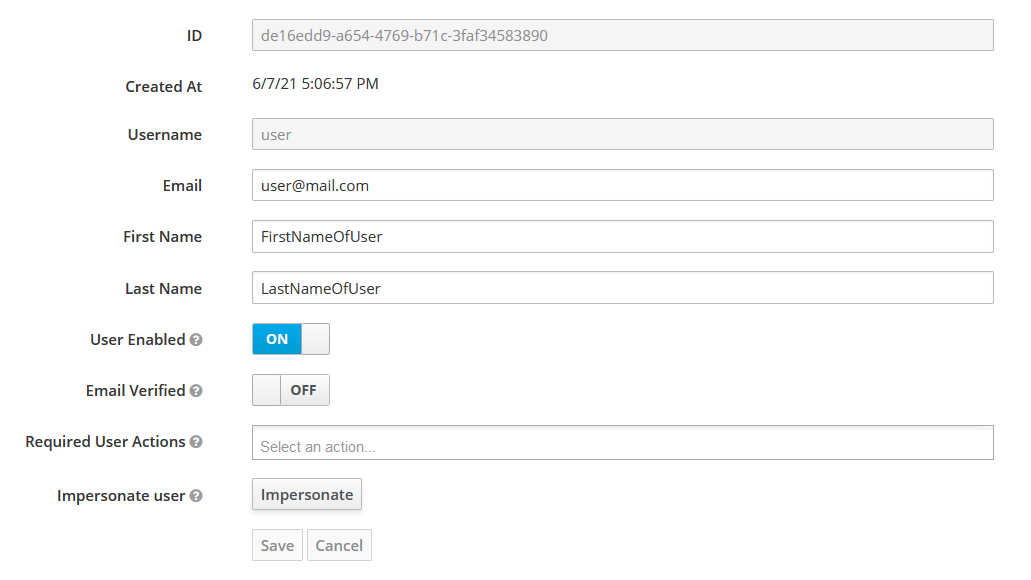
\includegraphics[width=1.0\textwidth]{gfx/keycloak-sample-user.PNG}
  \caption{Keycloak Sample User}
  \label{fig:chapter03:keycloak-sample-user}
 \end{figure}

In \autoref{fig:chapter03:keycloak-sample-user} Keycloak Sample User ist der erstellte Nutzer in Keycloak zu sehen. Neben 
den Standardattributen wird dem Nutzer auch eine Rolle zugewiesen, und zwar die Rolle ROLE\_USER.\bigskip

\begin{figure}[htbp]
  \centering
  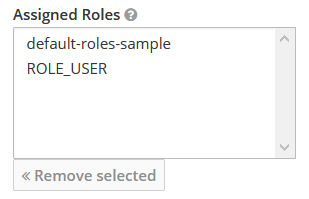
\includegraphics[width=0.5\textwidth]{gfx/keycloak-sample-user-role.PNG}
  \caption{Keycloak Sample User Role}
  \label{fig:chapter03:keycloak-sample-user-role}
 \end{figure}

Dies ist in Keycloak möglich und damit lässt sich in den Applikationen dann eine 
rollenbasierte Zugriffskontrolle realisieren, siehe Zugriffskontrolle. In \autoref{fig:chapter03:keycloak-sample-user-role} sind die zugewiesenen Rollen zu sehen. default-roles-sample ist eine durch Keycloak automatisch 
zugewiesene Rolle und hat hier keine weitere Relevanz. 
Außerdem wurde diesem Nutzer noch eine Gruppenzugehörigkeit und ein weiteres Attribut 
hinzugewiesen. Gruppenzugehörigkeiten sind in Firmen oftmals die Bürostandorte, 
Abteilungen und dergleichen. Nach Gruppenzugehörigkeiten wird in der Regel nicht 
autorisiert, denn dafür sind Rollen zuständig. Die Gruppenzugehörigkeit und das weitere 
Sample-Attribut hat hier nur den Sinn, dass es den Token umfangreicher macht und dies 
dient dazu, realistische Testbedingungen zu schaffen. Der Nutzer ist also in der Gruppe 
Users und hat als zusätzliches Attribut das statische Schlüssel-Wert-Paar Attribute1:UserAttribute1. 
Zusätzlich musste in Keycloak ein Client registriert werden. Der Client ist diejenige 
Komponente im OAuth2 System, die den Token von dem Authorization Server, also 
Keycloak, erhält und den Token nutzt, um Zugriff auf Schnittstellen des Ressource Servers 
zu erhalten. Für den Authorization Code Grant ist mindestens eine Client-ID notwendig. In 
diesem Fall wurde ein sogenannten confidential client in Keycloak registriert. Dieser muss 
sich mit seinen Daten, also Client-ID und Client Secret, bei Keycloak authentifizieren, um 
Token zu erhalten.
